\section{Introduction} 
	This document s the user manual of \textit{Soldino}, a project by 
	\textit{8Lab Solutions} based on the Erhereum infrastructure. 
	\textit{Soldino} is a platform, managed by the Government, that allows 
	users to buy good and services and allows business to manage the VATs 
	related to those products.
	More precisely:
	\begin{itemize}
		\item citizens can:
		\begin{itemize}
			\item  buy goods and services;
		\end{itemize}
		\item Business can:
		\begin{itemize}
			\item sell goods and services;
			\item buy goods and services;
			\item manage VAT;
		\end{itemize}
		\item Government can:
		\begin{itemize}
			\item activate new users;
			\item deactivate existing users;
			\item mint Cubits;
			\item distribute Cubits;
			\item reimburse business of their VAT credit;
		\end{itemize}
	\end{itemize}

\section{Requiremets}
	To be able to use \textit{Soldino} you must have the latest version one 
	of the following browsers:
	\begin{itemize}
		\item Google Chrome;
		\item Mozilla Firefox.
	\end{itemize}
	You also must have the MetaMask plugin installed in your browser.
\subsection{MetaMask}
	\subsubsection{Installation}
	Before entering \textit{Soldino} check if you have MetaMask, a bridge between 
	your browser and the Ethereum network, installed. 
	If you don't, visit \url{https://metamask.io} to download it.\newline
	\begin{figure}[H]
		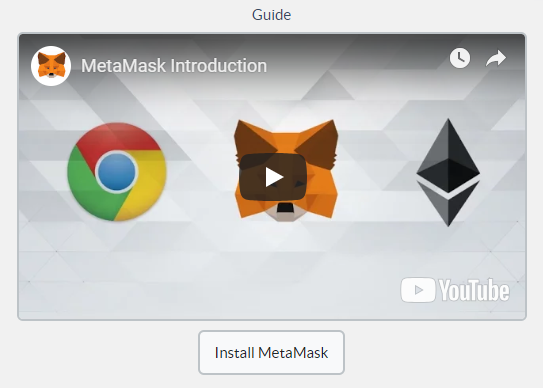
\includegraphics[width=5cm]{res/images/MetaMask_download.png}
		\centering
		\caption{MetaMask download page}
	\end{figure}
	\subsubsection{Configuration}
	After the installation process is complete you will see MetaMask's icon 
	on the top right of your browser, click it to set up your personal wallet.\\
	You can either create a new one or import an existing one from the 12 
	words seed phrase.
	\begin{figure}[H]
		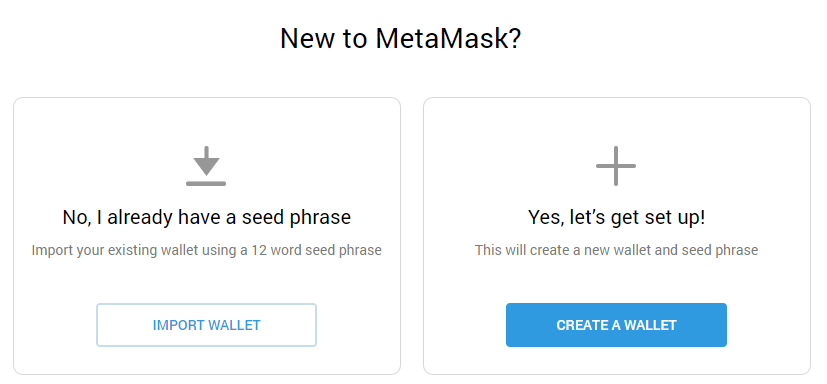
\includegraphics[width=5cm]{res/images/MetaMask_select.png}
		\centering
		\caption{MetaMask setup}
	\end{figure}
	\noindent After setting up your account you'll be able to join and use \textit{Soldino}.
	\newline \\
	Note that MetaMask has to be installed in your browser as long a you want 
	to use the platform.
	\subsubsection{Transactions}
	Every time you make a transaction MetaMask will show you its price and you'll
	be able to accept it or decline it.
	%PLACEHOLDER fot esempio transazione